\begin{surferPage}[D4+- Singularity]{$D_4^{+-}$ Singularity}
	The surface with the equation
	\[
		x^2y+y^3-z^2=0.
	\]
	corresponds to the so-called $D_4^{+-}$ singularity. This is the surface variant of three distinct straight lines meeting in a point, two of which cannot be seen in the real world, but only in a space with complex numbers. Plugging $z=0$ into the equation yields the plane curve with equation $x^2y+y^3=0$ which is equivalent to the union of one real and two non-real straight lines: $y\cdot(x-iy)\cdot(x+iy)=0$, with $i=\sqrt{-1}$ the imaginary unit.
	\vspace{-3ex}% subject to change in each translation
	\begin{Centering*}%
		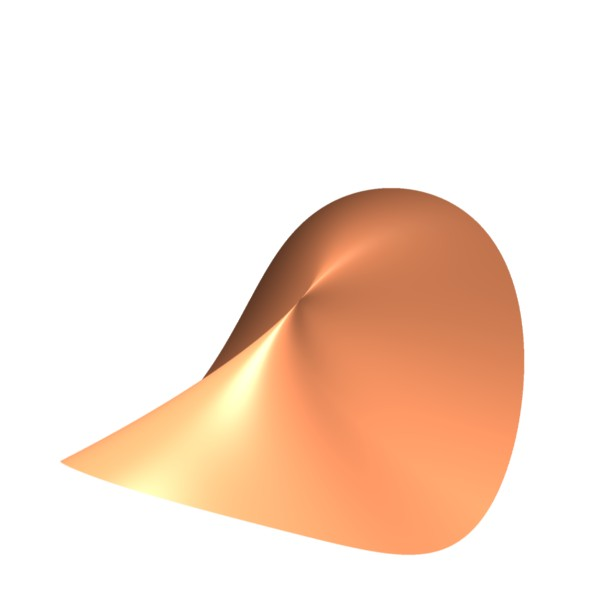
\includegraphics[width=1.2cm]{../../common/images/D4pm}\qquad%
		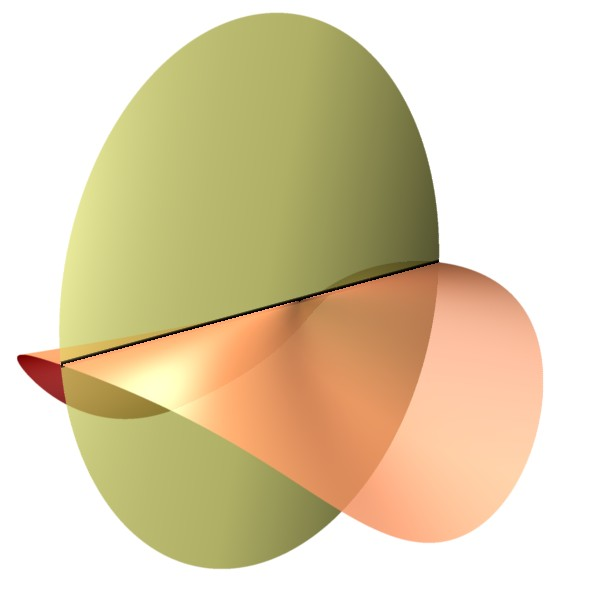
\includegraphics[width=1.2cm]{../../common/images/D4pm_def_with_plane_cut_0}%
	\end{Centering*}
	It is difficult to visualize the geometry of this singularity in our real world since an essential part only lives in the complex world. One attempt is to take the deformation
	\[
		(y+a)\cdot(x^2+y^2)+by^2-z^2=0,
	\]
	which yields the original equation for $a=b=0$:
	\vspace{-1ex}% subject to change in each translation
	\begin{Centering*}
		\begin{tabular}{c@{\quad}c@{\quad}c}
			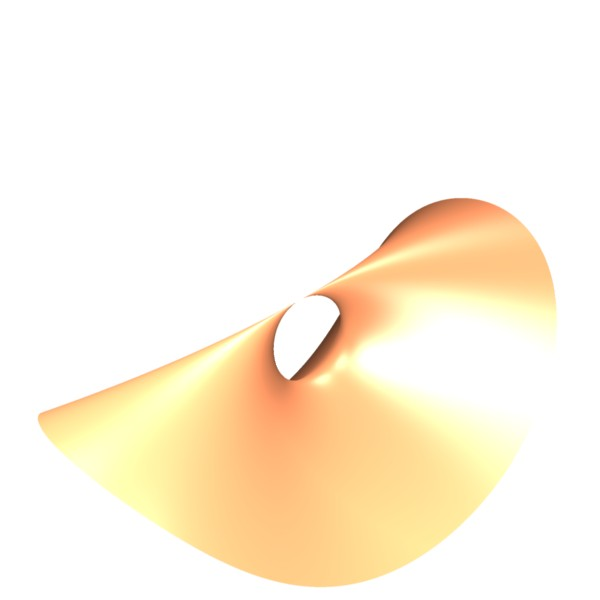
\includegraphics[width=1.2cm]{../../common/images/D4pm_1} &
			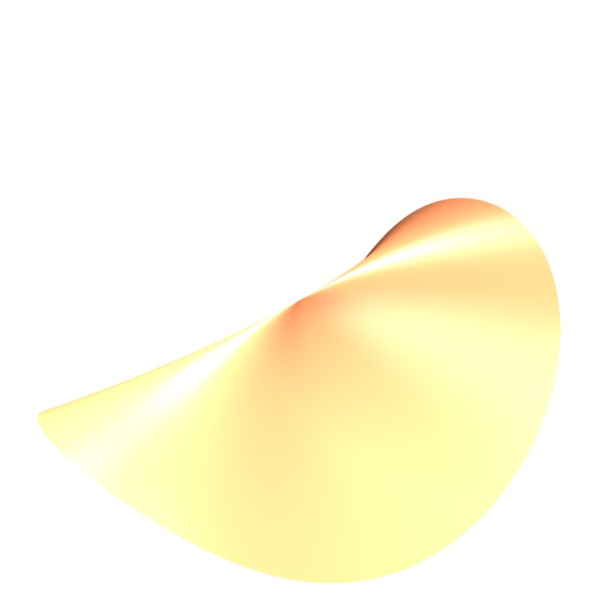
\includegraphics[width=1.2cm]{../../common/images/D4pm_0} &
			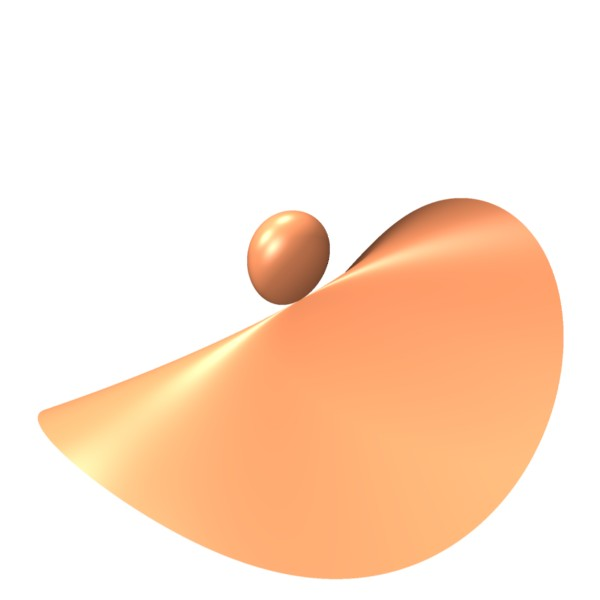
\includegraphics[width=1.2cm]{../../common/images/D4pm_2}\\
			$b=-0.5$ &
			$b=0$ &
			$b=0.5$
		\end{tabular}
	\end{Centering*}
\end{surferPage}
